\documentclass{article}
\usepackage{graphicx}
\usepackage{listings}
\usepackage{xcolor}

\definecolor{codegray}{gray}{0.9}
\lstdefinestyle{mystyle}{
    backgroundcolor=\color{codegray},
    basicstyle=\ttfamily,
    frame=single,
    breaklines=true
}
\lstset{style=mystyle}

\title{Network Scanning Experiment: Scan Your Home Network Using Nmap}
\author{Priyanshu Kumar Sharma, 2022-B-17102004A, B.Tech CTIS, SEM-VI/B}
\date{\today}

\begin{document}

\maketitle

\section{Objective}
To perform a basic scan of your home network using Nmap (Network Mapper) to identify active devices and open ports.

\section{Steps to Perform the Experiment}

\subsection{Step 1: Install Nmap (If Not Installed)}
Nmap is available for Windows, Linux, and macOS. Follow the instructions below to install it.

\textbf{Command:}
\begin{lstlisting}
nmap --version
\end{lstlisting}
\textbf{Description:} This command checks if Nmap is installed on your system and displays its version.

\begin{figure}[h]
    \centering
    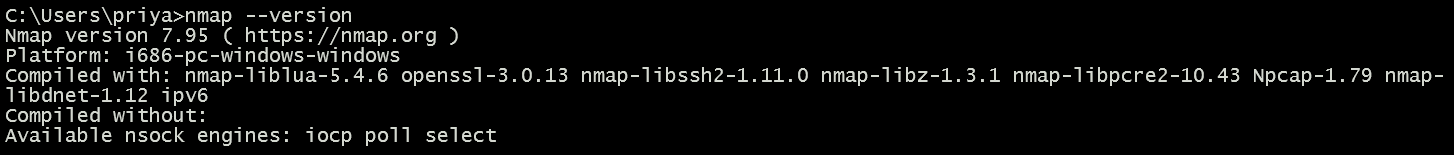
\includegraphics[width=1.0\textwidth, height=1.0\textheight, keepaspectratio]{images/nmap_version.png}
    \caption{Checking Nmap version}
\end{figure}

\subsection{Step 2: Identify Your Home Network IP Range}
To perform scanning, first identify your local IP address and subnet.

\textbf{Windows Command:}
\begin{lstlisting}
ipconfig
\end{lstlisting}
\textbf{Linux/macOS Command:}
\begin{lstlisting}
ifconfig
\end{lstlisting}
\textbf{Description:} These commands display network details, including your local IP address and subnet.

\begin{figure}[h]
    \centering
    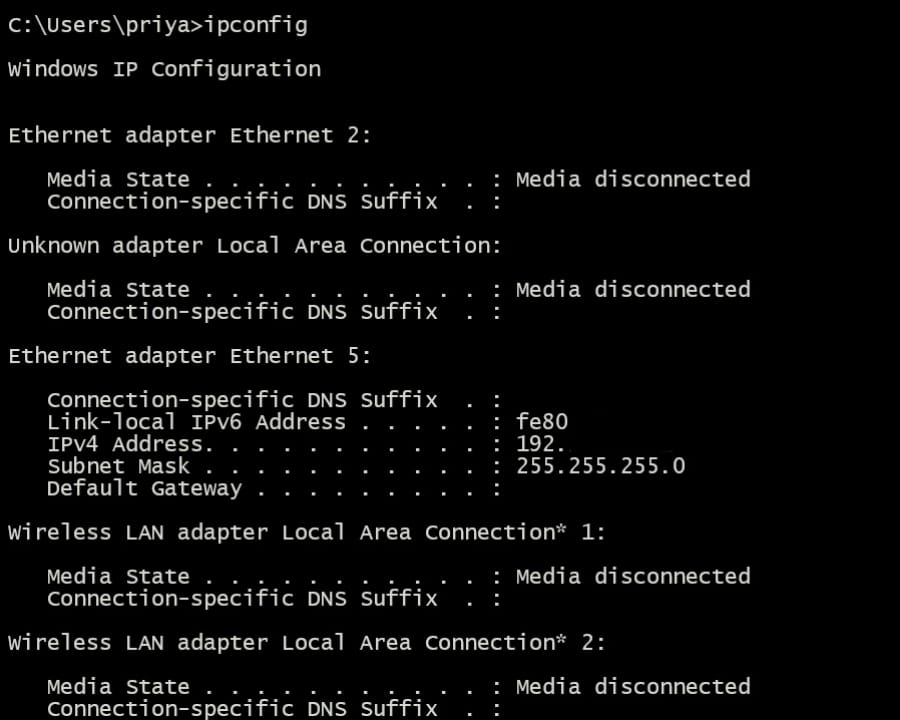
\includegraphics[width=0.8\textwidth]{images/ipconfig_ifconfig.png}
    \caption{Finding local IP address}
\end{figure}

\textbf{Check system availability}
\begin{lstlisting}
ping 10.11.217.229
\end{lstlisting}

\begin{figure}[h]
    \centering
    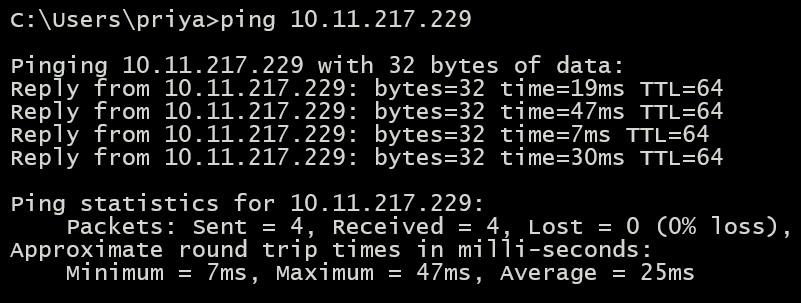
\includegraphics[width=0.8\textwidth]{images/ping.png}
    \caption{This checks if the device is available}
\end{figure}

\subsection{Step 3: Perform Basic Network Scan}
A simple scan to detect all active devices on your network.

\textbf{Command:}
\begin{lstlisting}
nmap -sn 10.11.217.229
\end{lstlisting}
\textbf{Description:} This scans all devices on the network without probing ports.

\begin{figure}[h]
    \centering
    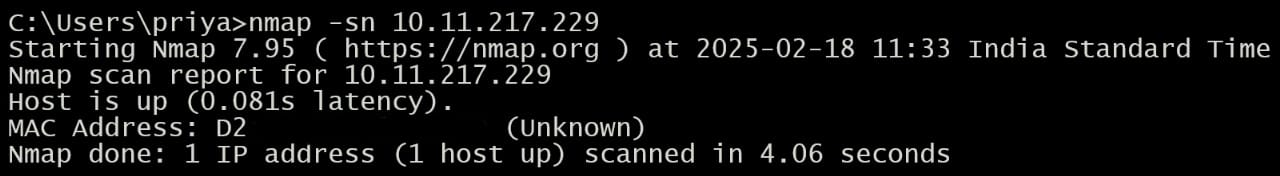
\includegraphics[width=0.8\textwidth]{images/nmap_scan.jpg} 
    \caption{Basic network scan}
\end{figure}

\subsection{Step 4: Perform a Port Scan on a Device}
To check open ports on a specific device (e.g., router).

\textbf{Command:}
\begin{lstlisting}
nmap -p- 10.11.217.229
\end{lstlisting}
\textbf{Description:} This scans all (0-65535) ports of the target device.

\begin{figure}[h]
    \centering
    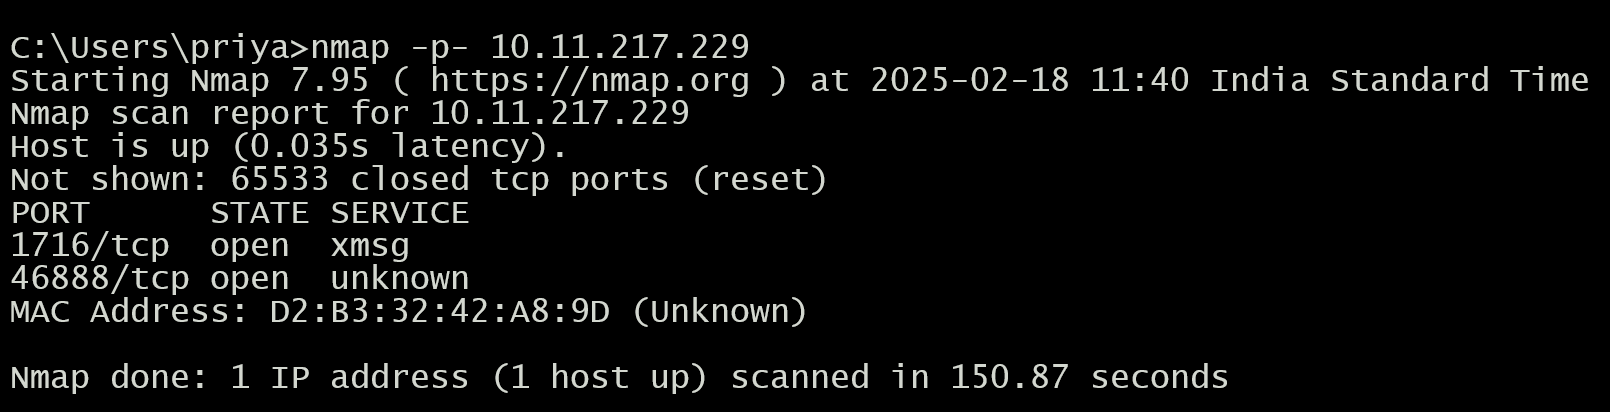
\includegraphics[width=0.8\textwidth]{images/port_scan.png}
    \caption{Scanning ports of a device}
\end{figure}

\subsection{Step 5: Detect Services and OS}
To get detailed information about a device.

\textbf{Command:}
\begin{lstlisting}
nmap -A 10.11.217.229
\end{lstlisting}
\textbf{Description:} This detects services (HTTP, SSH, etc.), operating system, and uptime.

\begin{figure}[h]
    \centering
    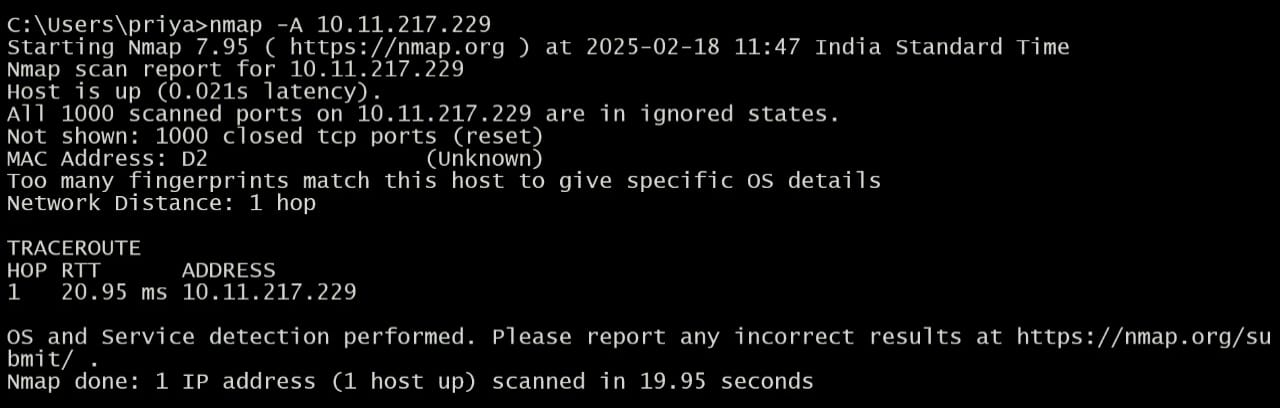
\includegraphics[width=0.8\textwidth]{images/service_detection.jpg}
    \caption{Detecting services and OS}
\end{figure}

\subsection{Step 6: Scan for Vulnerabilities (Optional \\& Ethical Use Only)}
To check for common vulnerabilities on a device.

\textbf{Command:}
\begin{lstlisting}
nmap --script vuln 10.11.217.229
\end{lstlisting}
\textbf{Description:} This scans for known vulnerabilities in the target system.

\begin{figure}[h]
    \centering
    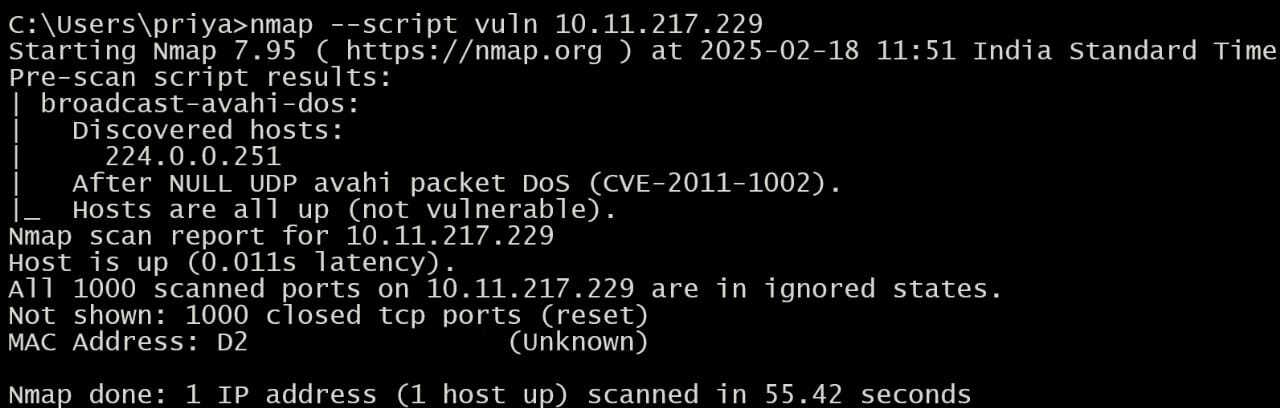
\includegraphics[width=0.8\textwidth]{images/vuln_scan.jpg}
    \caption{Scanning for vulnerabilities}
\end{figure}

\section{Precautions \\& Ethical Considerations}
\begin{itemize}
    \item Use Nmap only on networks you own or have permission to scan.
    \item Scanning unknown networks without authorization is illegal.
    \item Avoid aggressive scanning on shared networks (e.g., school, work).
    \item Ensure your firewall or security software allows scanning if needed.
\end{itemize}

\end{document}
